\documentclass[11pt,a4paper]{article}

% ---------------------------------------------------------------------------
% Packages (all available on Overleaf; compile with pdfLaTeX + BibTeX)
% ---------------------------------------------------------------------------
\usepackage[T1]{fontenc}
\usepackage[utf8]{inputenc}
\usepackage{lmodern}
\usepackage[margin=2.5cm]{geometry}
\usepackage{amsmath}
\usepackage{graphicx}
\usepackage{booktabs}
\usepackage{tabularx}
\usepackage{array}
\usepackage{float}
\usepackage{caption}
\usepackage{xcolor}
\usepackage{tikz}
\usetikzlibrary{positioning,arrows.meta,fit}
\usepackage{enumitem}
\usepackage{url}
\usepackage[hidelinks]{hyperref}

\definecolor{crimson}{HTML}{7F011F}
\definecolor{parchment}{HTML}{F5EBD0}
\captionsetup{font=small,labelfont=bf}
\setlist{itemsep=2pt,topsep=4pt}
\newcommand{\code}[1]{\texttt{#1}}

% ---------------------------------------------------------------------------
\title{A Rule-Based Expert System for Detecting Cheaters\\on a Counter-Strike 2 Leaderboard}
% TODO: replace with your name, student ID, course and instructor.
\author{Your Name \\ Student ID \\[4pt] \small Introduction to Artificial Intelligence, 5th Semester}
\date{\today}

\begin{document}
\maketitle

\begin{abstract}
Cheaters distort public leaderboards in competitive games. This project builds an expert system that
reads per-player match statistics from Counter-Strike 2 (CS2), diagnoses the likely kind of cheat,
and decides what to do about each player. Anti-cheat knowledge is written as Prolog rules and kept
separate from a domain-independent inference engine that uses forward chaining, backward chaining
and MYCIN certainty factors. The system acts on its own only for actions that can be undone
(monitor, hide from the leaderboard); a ban always goes to a human moderator together with the
system's full reasoning. Thresholds for ``abnormal'' play are set from matches without cheaters only,
and the system is tested on held-out players with real cheater labels from the CS2CD dataset. When
the system flags a player, 86--89\% of the flagged players are labelled cheaters, while only 0.5--2\%
of unlabelled players are flagged. It finds 41\% of labelled cheaters at its most sensitive setting.
A Streamlit console lets a moderator review cases, change the decision thresholds and consult the
system about any player they describe.
\end{abstract}

% ===========================================================================
\section{Introduction}
% ===========================================================================

A leaderboard ranks players by performance. When cheaters are on it, honest players lose their
places, and players trust the ranking less. Game companies use client-side anti-cheat software, but some
cheats get through, so leaderboards also need a second check based on what players actually did in
their matches.

This project builds that second check as an \emph{expert system}: a program that stores an expert's
knowledge as explicit rules and reasons with them the way the expert would. A human anti-cheat
moderator looks for signs such as aim that is too precise, too many kills through walls, or a player
who is far better than everyone else in the lobby. They weigh these signs against each other and
also against evidence that the player is simply very good. They then decide whether to watch the
player, hide them, or ban them. The system copies this process.

The course asks for four capabilities, and the system provides each one:
\begin{itemize}
  \item \textbf{Inference}: forward chaining turns match statistics into symptoms; backward
        chaining proves diagnoses from those symptoms.
  \item \textbf{Diagnostics}: the system names the likely cheat (aimbot, wallhack, rage cheat) with a
        certainty factor, and recognises legitimate strong players.
  \item \textbf{Decision making}: the system takes reversible actions on its own.
  \item \textbf{Decision support}: for a ban, the system only recommends. A moderator sees the
        evidence and the reasoning, and decides.
\end{itemize}

No machine learning is used. Every rule is written by hand, and the cheater labels in the
dataset are used only to test the system at the end.

% ===========================================================================
\section{Background}
% ===========================================================================

\subsection{Expert systems}
A classic expert system has a \emph{knowledge base} of if--then rules, a \emph{working memory} of
facts about the current case, an \emph{inference engine} that applies the rules to the facts, and an
\emph{explanation facility} that shows how a conclusion was reached
\cite{giarratano2005,russell2020}. Keeping the knowledge apart from the engine means the rules can be
read, checked and changed without touching the reasoning code.

\emph{Forward chaining} starts from the facts and fires every rule whose conditions hold, until no new
facts appear. It suits turning raw data into higher-level facts. \emph{Backward chaining} starts from
a goal, such as ``is this player cheating?'', and works back through the rules to the evidence it
needs. It suits diagnosis \cite{russell2020}.

\subsection{Certainty factors}
Anti-cheat evidence is rarely certain. MYCIN, an expert system for diagnosing blood infections,
handled this with \emph{certainty factors} (CFs) \cite{shortliffe1975,buchanan1984}. A CF is a
degree of belief between $-1$ (definitely false) and $+1$ (definitely true), with $0$ meaning no
evidence. CFs are not probabilities: the CFs of different diagnoses do not have to add up to 1. The
calculation used in this project is given in Section~\ref{sec:cf}.

% ===========================================================================
\section{Data}
% ===========================================================================

\subsection{The CS2CD dataset}
The system uses CS2CD \cite{cs2cd2025}, released with the AntiCheatPT paper
\cite{anticheatpt2025}. It contains 795 CS2 matches: 317 with at least one cheater and 478 with none.
Cheater labels are given \emph{per player}, which makes it possible to measure precision and recall.
Each match comes as a JSON file of game events (kills, damage, shots, flashes) and a Parquet file of
tick-level positions.

An expert system reasons over per-player facts, not over 64 position samples per second, so only
the JSON event files were downloaded (1.8\,GB instead of 51\,GB). Player IDs are anonymised per match
(\code{Player\_1} to \code{Player\_10}), so a player cannot be followed across matches. The unit of
analysis is therefore one \emph{player-match}: 7,925 of them, 1,309 labelled as cheaters, with 91,576
kills.

\subsection{Fact extraction}
Python turns each match into base facts, the system's working memory. It counts and does nothing
else: no rates, no judgements. For every player-match it writes ten \code{stat/3} facts (rounds,
kills, deaths, assists, shots, gun hits, head hits, damage, flash assists, enemies flashed), and for
every kill one \code{kill/9} fact recording whether it was a headshot, through smoke, through a wall,
while flashed, while airborne, and the distance. Warm-up events, bots, grenades and knives are left
out of the shot counts, and shotguns are excluded from accuracy because one shot fires many pellets.
The cheater label is never written into the facts.

One data problem was found and fixed during this step. On a killing blow the event field
\code{dmg\_health} reports the full weapon damage including \emph{overkill} (up to 4,999), not the
health actually removed. This had pushed damage per round as high as 1,179, which is impossible. The
extractor now tracks each victim's health from spawn and credits only the health that was removed.
After the fix, the median clean player deals 73.6 damage per round.

% ===========================================================================
\section{System architecture}
% ===========================================================================

Figure~\ref{fig:architecture} shows the parts of the system. Python handles data and the user
interface. Everything that reasons about a player happens in SWI-Prolog \cite{swipl2012}, reached
from Python through the \code{pyswip} library.

\begin{figure}[H]
\centering
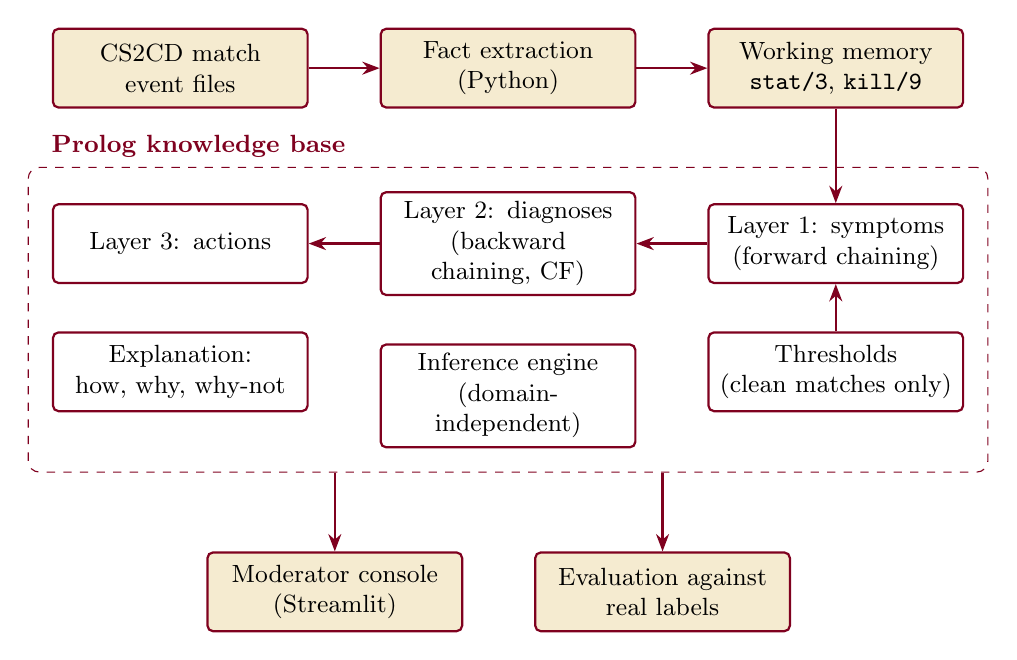
\begin{tikzpicture}[
    box/.style={draw=crimson, thick, rounded corners=2pt, fill=parchment, align=center,
                minimum height=10mm, text width=30mm, font=\small},
    kb/.style={box, fill=white},
    arr/.style={-{Stealth[length=2.2mm]}, thick, crimson},
    node distance=6mm and 9mm]
  \node[box] (json) {CS2CD match\\event files};
  \node[box, right=of json] (facts) {Fact extraction\\(Python)};
  \node[box, right=of facts] (wm) {Working memory\\\code{stat/3}, \code{kill/9}};

  \node[kb, below=12mm of wm] (sym) {Layer 1: symptoms\\(forward chaining)};
  \node[kb, left=of sym] (diag) {Layer 2: diagnoses\\(backward chaining, CF)};
  \node[kb, left=of diag] (act) {Layer 3: actions};
  \node[kb, below=of sym] (thr) {Thresholds\\(clean matches only)};
  \node[kb, below=of diag] (eng) {Inference engine\\(domain-independent)};
  \node[kb, below=of act] (exp) {Explanation:\\how, why, why-not};

  \node[draw=crimson, dashed, rounded corners, inner sep=3mm, fit=(sym)(diag)(act)(thr)(eng)(exp),
        label={[font=\small\bfseries, text=crimson]above left:Prolog knowledge base}] (kbbox) {};

  \node[box, below=10mm of kbbox.south, xshift=-22mm] (ui) {Moderator console\\(Streamlit)};
  \node[box, right=of ui] (ev) {Evaluation against\\real labels};

  \draw[arr] (json) -- (facts);
  \draw[arr] (facts) -- (wm);
  \draw[arr] (wm) -- (sym);
  \draw[arr] (thr) -- (sym);
  \draw[arr] (sym) -- (diag);
  \draw[arr] (diag) -- (act);
  \draw[arr] (kbbox.south -| ui.north) -- (ui);
  \draw[arr] (kbbox.south -| ev.north) -- (ev);
\end{tikzpicture}
\caption{Architecture. Python extracts facts and draws the console; all reasoning is done by the
Prolog knowledge base and its inference engine.}
\label{fig:architecture}
\end{figure}

The Prolog code is split by role:
\begin{itemize}
  \item \code{engine.pl}, the inference engine: forward chaining, backward chaining with
        certainty factors. It contains no knowledge about CS2.
  \item \code{metrics.pl}: the single definition of every metric and of how much data each metric
        needs.
  \item \code{thresholds.pl}: what counts as abnormal, generated by calibration.
  \item \code{symptoms.pl}, \code{diagnosis.pl}, \code{actions.pl}: the three layers of rules.
  \item \code{explain.pl}: the explanation facility.
  \item \code{main.pl}: the entry point that loads all of the above.
\end{itemize}
Appendix~\ref{app:code} lists every source file and what it does.

% ===========================================================================
\section{The knowledge base}
% ===========================================================================

\subsection{Metrics and evidence requirements}
Ten metrics are defined in Prolog from the base facts (Table~\ref{tab:thresholds}). A rate means
little when it rests on too little data, so each metric has a minimum: headshot rate needs 20 gun
hits, accuracy needs 50 shots, per-round metrics need 8 rounds, and kill-type rates need 8 kills.
A player with no measurable aim metric gets the symptom \code{insufficient\_evidence}, and the system
takes no action on them instead of guessing.

\subsection{Calibration: what counts as abnormal}
\label{sec:calibration}
A symptom fires when a metric is unusually high compared with normal players. ``Normal'' is measured
on players from matches \emph{without} cheaters, never on cheaters, in the way a doctor's normal
range for blood pressure comes from healthy people. To keep the test fair, the 478 clean matches
are split in two. The even-numbered half sets the thresholds, and the odd-numbered half is kept for
testing. For each metric the system takes the 95th and 99th percentile of the calibration players
(Table~\ref{tab:thresholds}).

\begin{table}[H]
\centering
\small
\caption{Metrics and their thresholds, calibrated on players from the even-numbered clean matches.}
\label{tab:thresholds}
\begin{tabular}{llrrr}
\toprule
Metric & Meaning & p95 & p99 & Players \\
\midrule
Headshot rate     & share of gun hits that hit the head  & 0.373 & 0.716 & 1,960 \\
Accuracy          & share of gun shots that hit an enemy & 0.304 & 0.436 & 2,127 \\
Damage per round  & average damage per round             & 135.1 & 171.4 & 2,215 \\
Kills per round   & kills per round                      & 1.353 & 1.838 & 2,215 \\
Kill/death        & kills per death                      & 2.784 & 6.643 & 2,215 \\
Headshot kills    & share of kills that are headshots    & 0.800 & 0.917 & 1,796 \\
Wallbang kills    & share of kills through walls         & 0.222 & 0.792 & 1,796 \\
Smoke kills       & share of kills through smoke         & 0.154 & 0.250 & 1,796 \\
Kills while flashed & share of kills while blinded       & 0.088 & 0.136 & 1,796 \\
Airborne kills    & share of kills while in the air      & 0.042 & 0.125 & 1,796 \\
\bottomrule
\end{tabular}
\end{table}

Three alternatives were tried and rejected:
\begin{itemize}
  \item \textbf{99.9th percentile.} The ``clean'' matches contain cheaters nobody labelled: headshot
        rate jumps from 0.37 at p95 to 0.72 at p99, which a population of honest players does not
        produce. The 99.9th percentile is therefore set by unlabelled cheaters and was dropped.
  \item \textbf{Tukey fences} ($Q_3 + 3\cdot\mathrm{IQR}$). For metrics where most players score
        zero, such as airborne kills, the IQR is 0, so the threshold becomes 0 and flags up to 20\%
        of normal players.
  \item \textbf{Separate thresholds per match type.} Official and Premier matchmaking differ mostly
        in how many unlabelled cheaters they contain, not in normal play, and splitting would leave
        too few players per group.
\end{itemize}
Figure~\ref{fig:calibration} compares the calibration players with labelled cheaters.

\begin{figure}[H]
\centering
\includegraphics[width=0.92\textwidth]{figures/calibration.pdf}
\caption{Four metrics for calibration players (blue) and labelled cheaters (orange), with the p95
and p99 thresholds.}
\label{fig:calibration}
\end{figure}

\subsection{Layer 1: symptoms by forward chaining}
Forward rules are stored as data, \code{fr(Stratum, RuleId, Player, Symptom, CF, Evidence, Body)}.
The engine fires every rule whose body holds until no new symptom appears. Rules run in
\emph{strata}: a rule that checks that a symptom is \emph{absent} only runs after every rule that
could produce that symptom (stratified negation).
\begin{itemize}
  \item \code{s\_abnormal} (stratum 1): a metric above p99 gives \code{abnormal(M)} with CF 0.8;
        above p95 gives CF 0.4.
  \item \code{s\_insufficient} (stratum 1): no aim metric has enough data.
  \item \code{s\_high\_impact} (stratum 2): damage per round, kills per round or kill/death is
        abnormal; the CF is that of the strongest one.
  \item \code{s\_normal\_mechanics} (stratum 2): headshot rate and accuracy were both measured and
        neither is abnormal (CF 0.8).
\end{itemize}

\subsection{Layer 2: diagnoses by backward chaining}
Backward rules are \code{br(RuleId, Conclusion, Premises, RuleCF)} (Table~\ref{tab:rules}). To decide
whether a player is cheating, the engine looks for rules that conclude \code{cheating}, then proves
their premises (\code{aimbot}, \code{wallhack}, \code{rage\_cheat}, \code{legit\_outlier}) from their
own rules, down to the symptoms. The rule CFs are knowledge-engineering judgements. They were set
before any evaluation and were not tuned on the labels.

\begin{table}[H]
\centering
\small
\caption{Backward-chaining rules. A rule fires when every premise has CF above 0.2.}
\label{tab:rules}
\begin{tabular}{llp{7.6cm}r}
\toprule
Rule & Concludes & If all of & Rule CF \\
\midrule
a1 & aimbot & abnormal headshot rate, abnormal accuracy & 0.85 \\
a2 & aimbot & abnormal headshot rate, abnormal headshot-kill rate & 0.60 \\
a3 & aimbot & abnormal accuracy, high impact & 0.50 \\
a4 & aimbot & abnormal headshot rate, high impact & 0.50 \\
w1 & wallhack & abnormal wallbang rate & 0.50 \\
w2 & wallhack & abnormal wallbang rate, high impact & 0.70 \\
w3 & wallhack & abnormal smoke-kill rate, high impact & 0.30 \\
r1 & rage cheat & abnormal airborne-kill rate, abnormal headshot rate & 0.70 \\
r2 & rage cheat & abnormal flashed-kill rate, abnormal headshot rate & 0.50 \\
r3 & rage cheat & abnormal wallbang rate, headshot rate and accuracy & 0.80 \\
l1 & legit strong player & high impact, normal mechanics & 0.80 \\
c1--c3 & cheating & aimbot / wallhack / rage cheat & 1.00 \\
c4 & cheating & legit strong player & $-0.70$ \\
\bottomrule
\end{tabular}
\end{table}

Rule \code{c4} is evidence \emph{against} cheating. A player with very high impact but ordinary aim
looks like a strong honest player, and their cheating CF is reduced instead of raised.

\subsection{How certainty factors are calculated}
\label{sec:cf}
The engine follows MYCIN \cite{shortliffe1975}:
\begin{enumerate}
  \item A rule's premises are all required, so the rule is only as strong as its weakest premise:
        \[ \mathit{CF}_{\text{rule}} = \min_i \mathit{CF}(\text{premise}_i) \times \mathit{RuleCF}. \]
        The rule fires only if that minimum is above 0.2.
  \item Rules with the same conclusion are combined pairwise:
  \[
  \mathit{CF}(x,y) =
  \begin{cases}
    x + y(1-x) & x, y \ge 0 \\
    x + y(1+x) & x, y < 0 \\
    \dfrac{x+y}{1-\min(|x|,|y|)} & \text{otherwise.}
  \end{cases}
  \]
  Each new piece of supporting evidence closes part of the remaining gap to 1, so the result grows
  but never passes 1.
\end{enumerate}

Table~\ref{tab:cfexample} shows the calculation for an example player whose headshot rate (0.824),
accuracy (0.607), damage per round and kills per round are above p99, and whose kill/death and
headshot-kill rate are above p95.

\begin{table}[H]
\centering
\small
\caption{Worked example: the aimbot CF of the ``aimbot-like'' example player.}
\label{tab:cfexample}
\begin{tabular}{lllr}
\toprule
Rule & Premise CFs (weakest) & Contribution & Combined aimbot CF \\
\midrule
a1 & 0.8, 0.8 (0.8) & $0.8 \times 0.85 = 0.68$ & 0.680 \\
a2 & 0.8, 0.4 (0.4) & $0.4 \times 0.60 = 0.24$ & $0.680 + 0.24(1-0.680) = 0.757$ \\
a3 & 0.8, 0.8 (0.8) & $0.8 \times 0.50 = 0.40$ & $0.757 + 0.40(1-0.757) = 0.854$ \\
a4 & 0.8, 0.8 (0.8) & $0.8 \times 0.50 = 0.40$ & $0.854 + 0.40(1-0.854) = 0.912$ \\
\bottomrule
\end{tabular}
\end{table}

The aimbot CF of 0.91 then passes through rule \code{c1} (rule CF 1.0), so the player's cheating CF
is 0.91. As an example of evidence against, an aimbot CF of 0.40 combined with a legit-player
contribution of $-0.22$ gives $(0.40-0.22)/(1-0.22) = 0.23$.

\subsection{Layer 3: actions}
The cheating CF decides the action (Table~\ref{tab:actions}). The thresholds are Prolog facts
(\code{action\_threshold/2}), so the console can change them while it runs.

\begin{table}[H]
\centering
\small
\caption{Actions. Only actions that can be undone are taken automatically.}
\label{tab:actions}
\begin{tabular}{llll}
\toprule
Cheating CF & Action & Who decides & Capability \\
\midrule
no aim data & no action & automatic & decision making \\
below 0.20 & clear & automatic & decision making \\
0.20 or more & monitor & automatic & decision making \\
0.50 or more & hide from leaderboard & automatic & decision making \\
0.75 or more & ban review & human moderator & decision support \\
\bottomrule
\end{tabular}
\end{table}

\subsection{Explanation facility}
Every conclusion can be explained. \code{how/3} prints the proof tree, \code{why/2} explains the
action, and \code{why\_not/3} lists each rule for a conclusion with its weakest premise, so a
moderator can see why a cheat was \emph{not} diagnosed. An extract for the example player:

{\small
\begin{verbatim}
cheating: CF 0.91
  rule c1 (for, rule CF 1.00) contributes 0.91
    aimbot: CF 0.91
      rule a1 (for, rule CF 0.85) contributes 0.68
        abnormal(headshot_rate): CF 0.80, headshot_rate = 0.824 > p99 (0.716)
        abnormal(accuracy): CF 0.80, accuracy = 0.607 > p99 (0.436)
      rule a2 (for, rule CF 0.60) contributes 0.24
        abnormal(headshot_rate): CF 0.80, headshot_rate = 0.824 > p99 (0.716)
        abnormal(hs_kill_rate): CF 0.40, hs_kill_rate = 0.868 > p95 (0.800)
\end{verbatim}
}

% ===========================================================================
\section{The moderator console}
\label{sec:console}
% ===========================================================================

The console is a Streamlit web app. One dedicated worker thread owns the Prolog engine, because
SWI-Prolog must not be queried from several threads at once, and Streamlit runs each page refresh on
a different thread. The console has six views:
\begin{itemize}
  \item \textbf{Check a player}: the user enters one player's match numbers. They become temporary
        Prolog facts, the same knowledge base reasons over them, and the facts are removed
        afterwards. The answer is shown in four parts, one per capability (Figure~\ref{fig:check}).
        Each input field only accepts values a real match allows, given the fields before it. For
        example, deaths can be at most the number of rounds, and kills plus assists at most five per
        round.
  \item \textbf{Review queue}: players sent for a ban decision, most certain first, with the
        reasoning. The moderator confirms the ban, keeps the player hidden, or restores them, and
        each decision is logged (Figure~\ref{fig:queue}).
  \item \textbf{Leaderboard}: the public ranking. Players the system hid lose their rank; a
        moderator's decision overrides the system.
  \item \textbf{Player lookup}: any player's verdict with how, why and why-not explanations.
  \item \textbf{Strictness dial}: sliders that rewrite the action thresholds in Prolog and make the
        knowledge base decide again for every player, with live precision and recall
        (Figure~\ref{fig:dial}).
  \item \textbf{Knowledge base}: the rules and thresholds, read live from Prolog.
\end{itemize}

\begin{figure}[H]
\centering
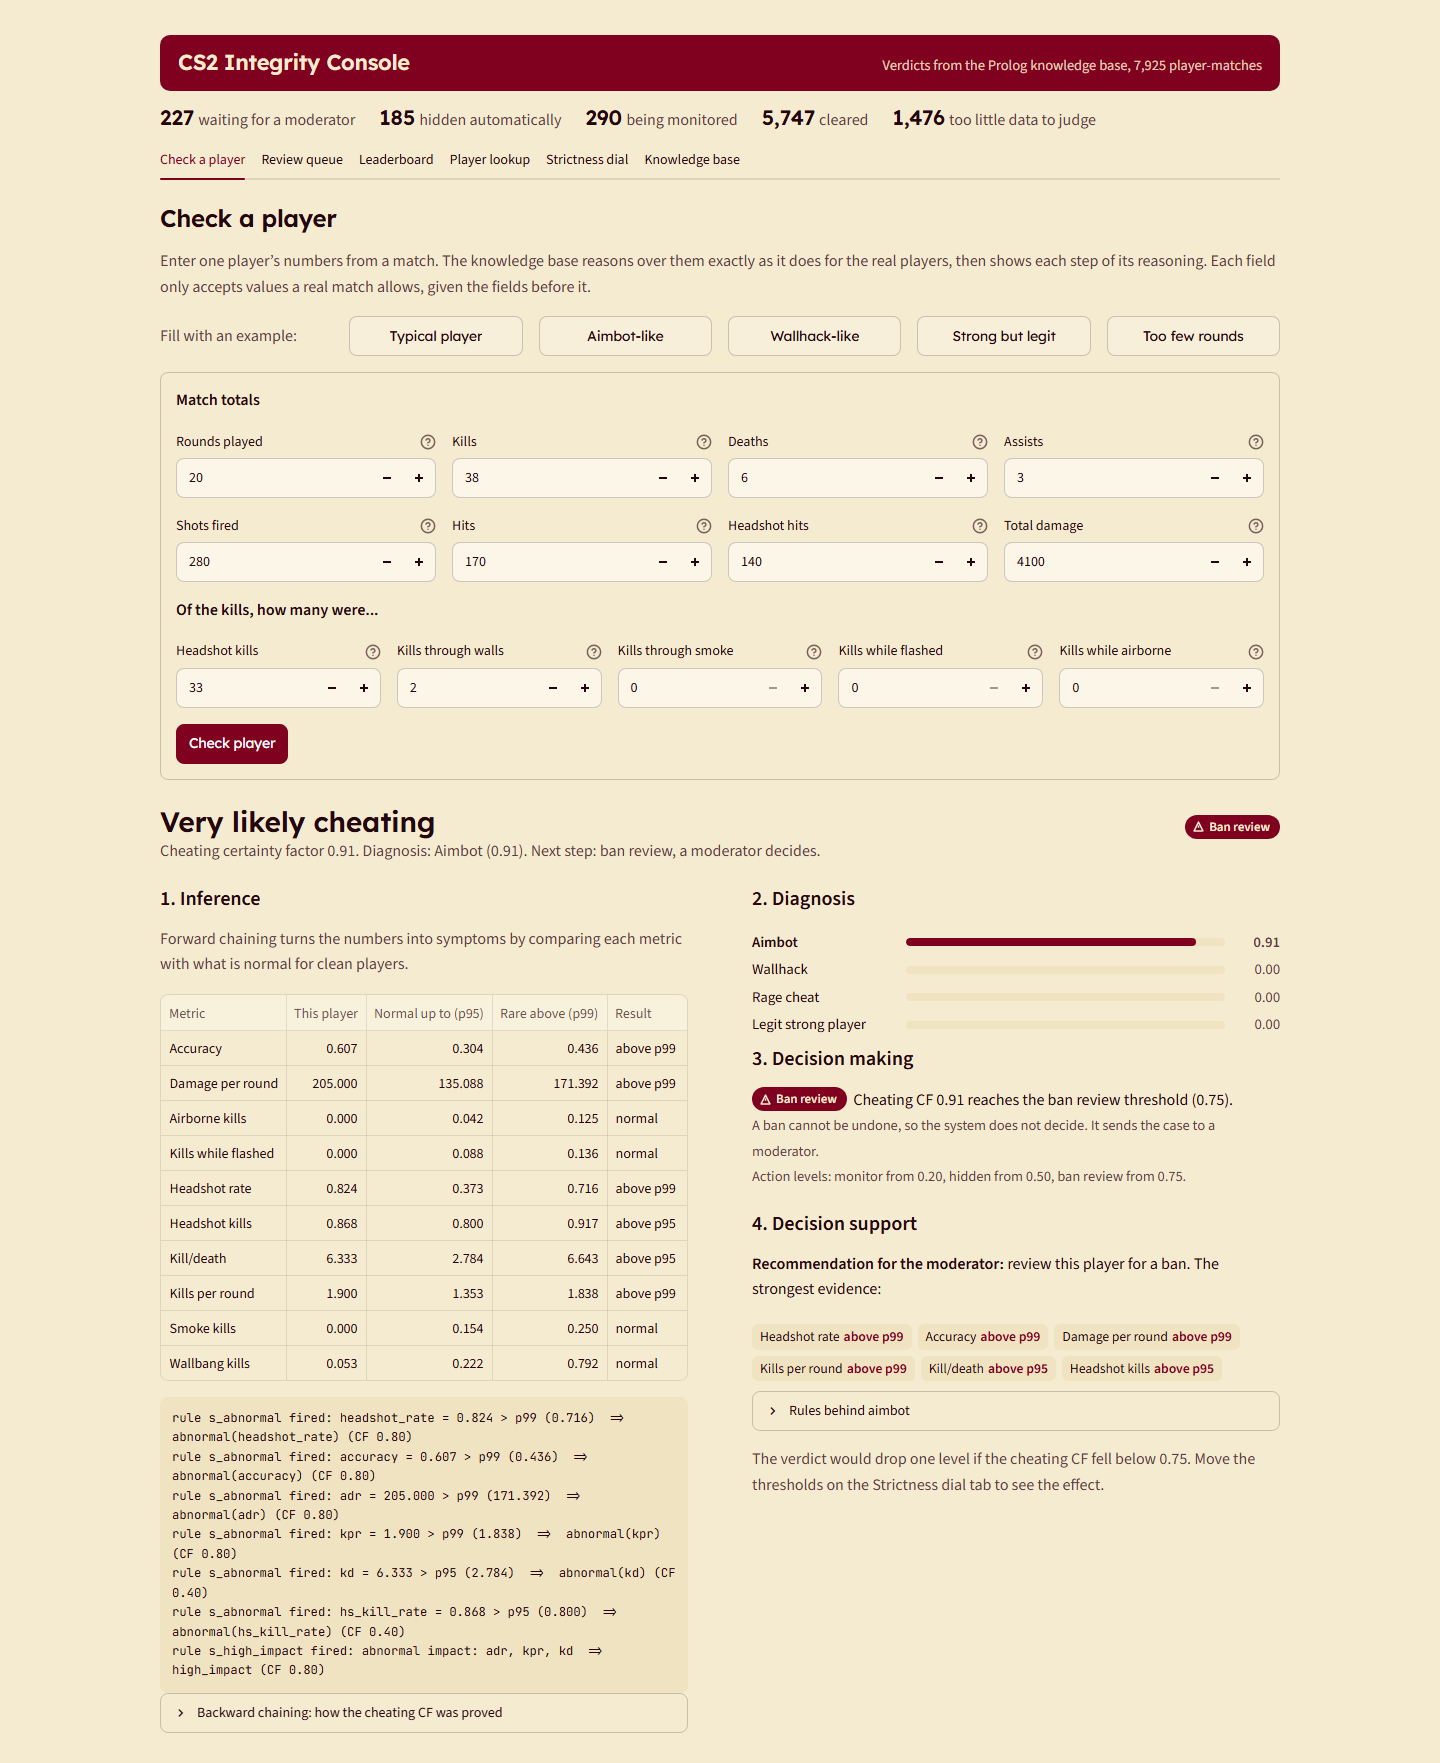
\includegraphics[width=0.88\textwidth]{screenshots/ui_check_player.png}
\caption{``Check a player'': the verdict for the aimbot-like example, split into inference,
diagnosis, decision making and decision support.}
\label{fig:check}
\end{figure}

\begin{figure}[H]
\centering
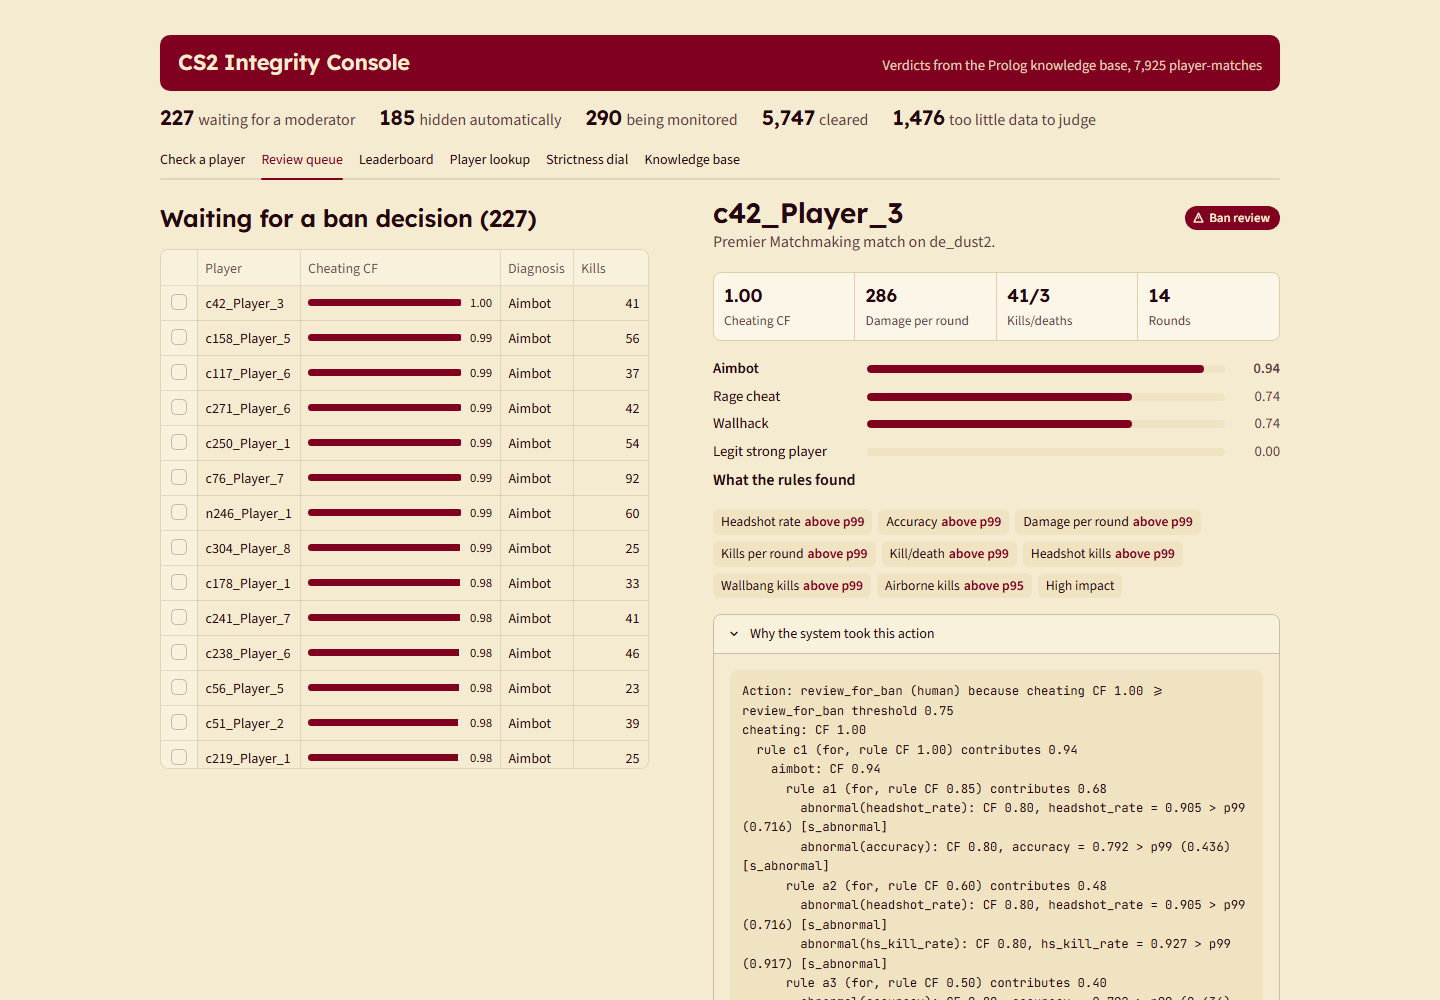
\includegraphics[width=0.88\textwidth]{screenshots/ui_review_queue.png}
\caption{Review queue. The moderator, not the system, decides on bans.}
\label{fig:queue}
\end{figure}

\begin{figure}[H]
\centering
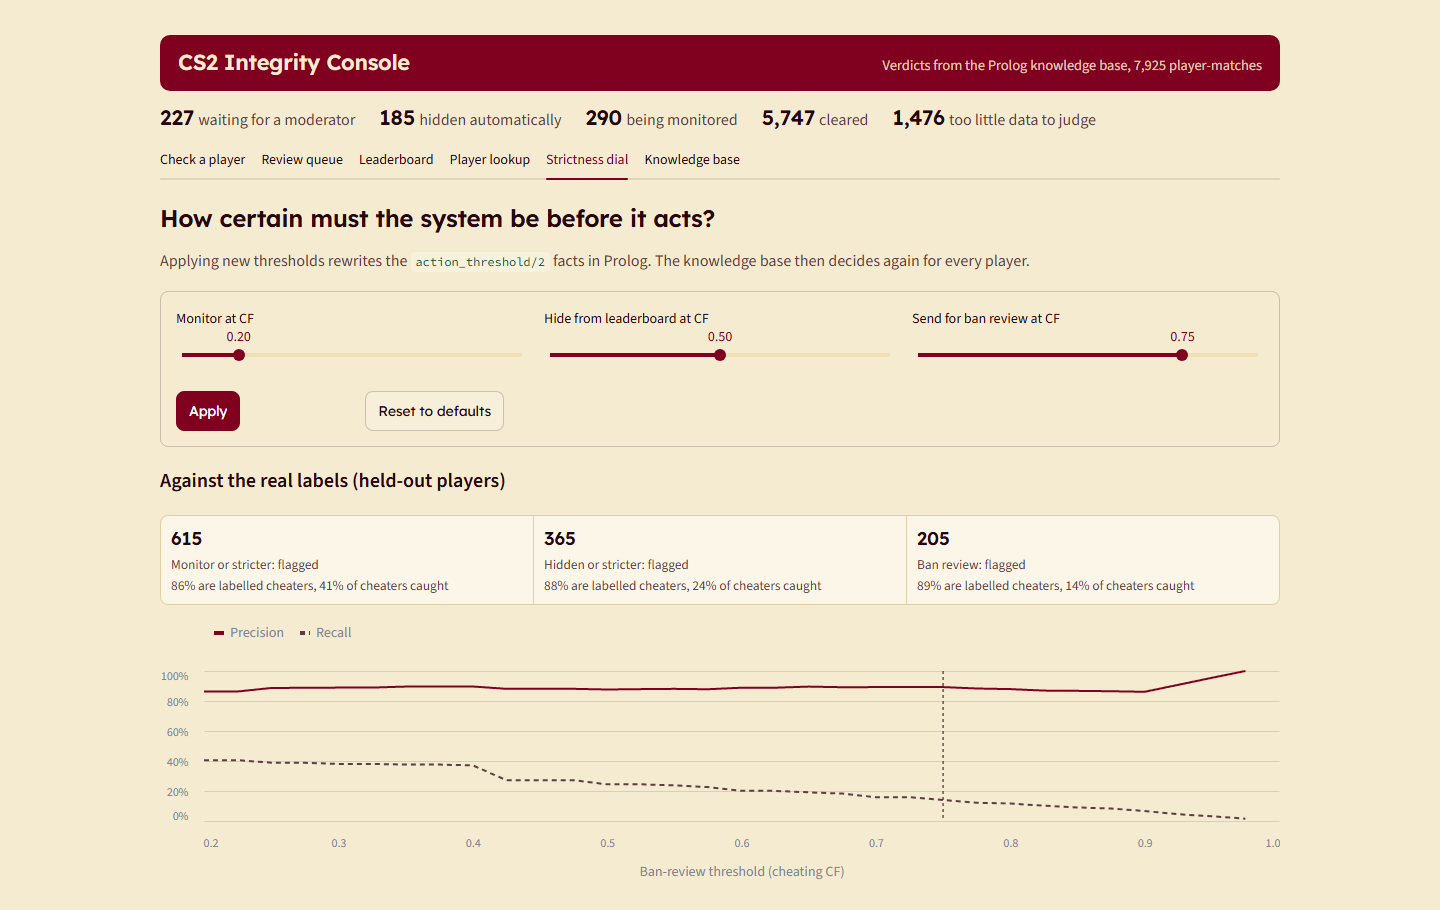
\includegraphics[width=0.88\textwidth]{screenshots/ui_strictness_dial.png}
\caption{Strictness dial. Changing a threshold makes the knowledge base decide again.}
\label{fig:dial}
\end{figure}

% ===========================================================================
\section{Evaluation}
% ===========================================================================

\subsection{Setup}
The system is tested on every player except those in the even-numbered clean matches used for
calibration: 5,540 player-matches, of which 1,309 are labelled cheaters (base rate 23.6\%). A player
counts as \emph{flagged} at three operating points: monitor or stricter, hide or stricter, and ban
review only. For comparison, three single-signal baselines flag a player when one symptom is present,
without a knowledge base.

One caveat applies to every number below. ``Not labelled'' does not mean ``honest'': the clean
matches contain cheaters nobody labelled (Section~\ref{sec:calibration}), so some flagged ``non-cheaters'' are likely
real cheaters, and the measured precision is a lower bound.

\subsection{Results}

\begin{table}[H]
\centering
\small
\caption{Operating points on the 5,540 held-out player-matches. FPR: share of unlabelled players
flagged.}
\label{tab:results}
\begin{tabular}{lrrrrr}
\toprule
Operating point & Flagged & Precision & Recall & F1 & FPR \\
\midrule
Expert system: monitor or stricter & 615 & 0.863 & 0.406 & 0.552 & 0.020 \\
Expert system: hide or stricter    & 365 & 0.877 & 0.244 & 0.382 & 0.011 \\
Expert system: ban review only     & 205 & 0.893 & 0.140 & 0.242 & 0.005 \\
\midrule
Baseline: headshot rate $>$ p95     & 561 & 0.797 & 0.341 & 0.478 & 0.027 \\
Baseline: any metric $>$ p99        & 714 & 0.793 & 0.432 & 0.560 & 0.035 \\
Baseline: any metric $>$ p95        & 1,653 & 0.529 & 0.668 & 0.590 & 0.184 \\
\bottomrule
\end{tabular}
\end{table}

Table~\ref{tab:results} and Figure~\ref{fig:pr} show the main results.
\begin{itemize}
  \item \textbf{When the system flags a player, it is usually right.} 86--89\% of flagged players
        are labelled cheaters, against a base rate of 24\%.
  \item \textbf{It is more precise than single signals.} At almost the same recall as the best
        baseline (0.41 against 0.43), it flags \emph{half} as many unlabelled players (2.0\% against
        3.5\%). Combining evidence with certainty factors, and counting legitimate strong play as
        evidence against, is what makes the difference.
  \item \textbf{It is cautious and misses many cheaters.} At most 41\% of labelled cheaters are
        flagged. This is acceptable for a system that recommends bans, but it is the main
        weakness.
\end{itemize}

\begin{figure}[H]
\centering
\includegraphics[width=0.7\textwidth]{figures/pr_curve.pdf}
\caption{Precision against recall. The dashed segment is the block of players with cheating CF 0,
for whom no rule fired.}
\label{fig:pr}
\end{figure}

\begin{figure}[H]
\centering
\includegraphics[width=0.92\textwidth]{figures/actions_by_label.pdf}
\caption{Actions taken for labelled cheaters and for unlabelled players.}
\label{fig:actions}
\end{figure}

Figure~\ref{fig:actions} shows where the missed cheaters go. A quarter of labelled cheaters (26\%)
played too little to measure their aim, so the system took no action. A further third (34\%) were
cleared. Their numbers looked normal, which is consistent with cheats that statistics alone cannot
see (Section~\ref{sec:limits}).

\paragraph{Where the false positives come from.} Of the 84 unlabelled players flagged at the most
sensitive setting, 69 come from matches without any labelled cheater. Those are the matches already
known to contain unlabelled cheaters, so many of these ``false'' flags are probably correct.

\paragraph{Rule quality.} Every rule that points to cheating is right 78--91\% of the time when it
fires (Figure~\ref{fig:rules}). The legit-strong-player rule \code{l1} fires mostly on unlabelled
players (79\%), which is its purpose.

\begin{figure}[H]
\centering
\includegraphics[width=0.85\textwidth]{figures/rules.pdf}
\caption{Share of labelled cheaters among the players each rule fired on.}
\label{fig:rules}
\end{figure}

\paragraph{Certainty factors and thresholds.} Figure~\ref{fig:cf} shows that labelled cheaters receive
much higher cheating CFs than unlabelled players. Figure~\ref{fig:dialcurve} shows the trade-off
behind the strictness dial: raising the ban-review threshold lowers recall, while precision stays
between 0.86 and 0.90 until the very top.

\begin{figure}[H]
\centering
\includegraphics[width=0.7\textwidth]{figures/cf_distribution.pdf}
\caption{Distribution of the cheating CF (log scale) for players with enough data.}
\label{fig:cf}
\end{figure}

\begin{figure}[H]
\centering
\includegraphics[width=0.7\textwidth]{figures/strictness_dial.pdf}
\caption{Precision and recall as the ban-review threshold moves.}
\label{fig:dialcurve}
\end{figure}

% ===========================================================================
\section{Limitations}
\label{sec:limits}
% ===========================================================================

\begin{itemize}
  \item \textbf{Where the knowledge comes from.} The rules encode general knowledge of how cheats
        behave (inhuman aim, kills through walls), not knowledge gathered from professional
        anti-cheat staff. A real system would need a knowledge-acquisition step with domain experts.
  \item \textbf{Label noise.} The clean matches contain unlabelled cheaters. This affects both the
        calibration (p99 is pushed up) and the evaluation (precision is underestimated).
  \item \textbf{Aggregated statistics miss subtle cheats.} A cheater who only uses a wallhack to
        know where enemies are, without shooting through walls, has normal statistics. Detecting
        that needs the tick-level position data this project left out.
  \item \textbf{Correlated evidence.} MYCIN treats rules as independent evidence, but rules
        \code{a1}, \code{a2} and \code{a4} all use the headshot rate, so one symptom is partly
        counted several times.
  \item \textbf{No player identity.} Players are anonymised per match, so the leaderboard ranks
        match performances rather than accounts, and cross-match cheats such as rank boosting cannot
        be detected.
  \item \textbf{Unrealistic cheater share.} 16.5\% of all player-matches are cheaters, and some
        lobbies contain eight or more. In a real player population precision would be lower.
\end{itemize}

% ===========================================================================
\section{Conclusion}
% ===========================================================================

The project shows that a classic rule-based expert system can do a useful part of leaderboard
anti-cheat work. Its knowledge is readable Prolog, its reasoning is forward and backward chaining
under MYCIN certainty factors, and every verdict comes with an explanation. It acts on its own only
when a mistake can be undone and leaves bans to a person. On real labelled data it is right
86--89\% of the time when it flags someone and flags half as many unlabelled players as the best
single-signal rule, at the cost of missing many cheaters.

Future work: acquire rules from anti-cheat experts; add knowledge based on positions and view
angles from the tick-level data; replace independent certainty factors with a method that handles
correlated evidence; and track players across matches once identities are available.

\bibliographystyle{plain}
\bibliography{references}

% ===========================================================================
\appendix
\section{Code structure}
\label{app:code}
% ===========================================================================

Table~\ref{tab:code} lists the source files. All reasoning lives in the Prolog files in \code{kb/};
the Python package \code{src/cheatdetect/} only reads data, moves facts in and out of Prolog,
evaluates the results and draws the console.

\begin{table}[H]
\centering
\small
\caption{Source files and what each one does.}
\label{tab:code}
\begin{tabularx}{\textwidth}{@{}>{\ttfamily}l X@{}}
\toprule
\normalfont\textbf{File} & \textbf{What it does} \\
\midrule
\multicolumn{2}{@{}l}{\textit{Knowledge base (\code{kb/}, SWI-Prolog)}} \\
main.pl        & Entry point; loads the other Prolog files in order. \\
engine.pl      & Domain-independent inference engine: forward chaining, backward chaining and
                 MYCIN certainty-factor combination. \\
metrics.pl     & Defines every metric (rates computed from \code{stat/3} and \code{kill/9} facts)
                 and the minimum data each metric needs. \\
thresholds.pl  & The p95/p99 values that count as abnormal; generated by \code{calibrate.py}. \\
symptoms.pl    & Layer 1: forward-chaining rules from metrics to symptoms. \\
diagnosis.pl   & Layer 2: backward-chaining rules from symptoms to diagnoses (aimbot, wallhack,
                 rage cheat, legitimate outlier), each with a certainty factor. \\
actions.pl     & Layer 3: maps a diagnosis to an action (monitor, hide from leaderboard, review
                 for ban) and decides whether the system may act alone. \\
explain.pl     & Explanation facility: \emph{how} a conclusion was reached, \emph{why} an action
                 was taken, \emph{why not} a conclusion did not fire. \\
\midrule
\multicolumn{2}{@{}l}{\textit{Python package (\code{src/cheatdetect/})}} \\
config.py         & All file and folder paths, in one place. \\
facts.py          & Fact extraction: parses the CS2CD event files and counts shots, hits, damage
                    and kills per player per match. Makes no judgements. \\
prolog\_io.py     & Writes the counts as Prolog facts (\code{stat/3}, \code{kill/9}) and loads the
                    knowledge base. The cheater label is never written. \\
calibrate.py      & Sets the thresholds from the calibration half of the clean matches and writes
                    \code{thresholds.pl}. \\
bridge.py         & Asks the knowledge base about every player and collects the answers (action,
                    CFs, diagnosis, explanation) into one table. \\
evaluate.py       & Compares the verdicts with the real labels on held-out players; produces the
                    figures and tables in this report. \\
kb\_service.py    & Runs every Prolog query on one worker thread, because SWI-Prolog cannot be
                    queried from several threads at once. \\
consultation.py   & Lets a user describe a player; the numbers become temporary facts, the same
                    knowledge base reasons over them, and the facts are removed afterwards. \\
moderation.py     & Records moderator decisions (ban, keep hidden, restore), which override the
                    system's automatic action. \\
\midrule
\multicolumn{2}{@{}l}{\textit{Other}} \\
app/streamlit\_app.py & The moderator console (Section~\ref{sec:console}). \\
scripts/download\_cs2cd.py & Downloads only the JSON event files of CS2CD. \\
scripts/build\_report.py   & Checks this report and packages it for Overleaf. \\
tests/            & Unit tests for every module above and for the knowledge base. \\
\bottomrule
\end{tabularx}
\end{table}

\end{document}
